% Womelsdorf Lab burst library user guide - Tutorial
% Written by Christopher Thomas.

\chapter{Tutorial}
\label{sect-tutorial}

%
%
%
\section{Reading and Processing Field Trip Data}
\label{sect-tutor-ft}

A minimal script for reading and processing Field Trip data using the wlBurst
library is given in Section \ref{sect-tutor-ftcode}. Steps that it performs
are described below:

\begin{itemize}
%
\item Libraries are added to the path.
%
\item Frequency bands of interest are defined.

The structure format used for this follows the same conventions as the
``\texttt{bandinfo}'' structure array in \texttt{WLNOTES.txt}.
%
\item Segmentation and parameter extraction configuration structures are
created. These use the conventions described in \texttt{SEGCONFIG.txt}
and \texttt{PARAMCONFIG.txt}, respectively.
%
\item Per-band overrides for segmentation and parameter extraction are
defined, per \linebreak \texttt{wlFT\_doFindEventsInTrials\_MT.m}.

These are intended to provide band-specific values for some of the fields
in the segmentation and parameter extraction configuration structures. The
sample code overrides several segmentation configuration fields but none
of the parameter extraction fields.

Tuning detection threshold (``\texttt{dbpeak}'') is particularly important.
A threshold that reliably detects events in one band may produce too many
false positives or fail to detect most events in another band.
%
\item The Field Trip data is loaded (in \texttt{ft\_datatype\_raw} format),
and is pruned to the desired subset of channels (the single channel
containing local field potential recordings, for the example dataset).
%
\item Metadata from a custom structure recording reward times is loaded
and converted into a data column in \texttt{trialinfo} within the Field Trip
data. This is then used to trim trials to exclude regions known to have
electrical artifacts.

The type of trimming that will be appropriate will vary widely from use case
to use case, but some type of trimming and/or time alignment will usually be
needed.
%
\item A 60 Hz notch filter is applied (FWHM 6~Hz, 20th order). This is
intended to remove electrical artifacts due to power line noise at US power
frequencies that existed in this dataset.

The use of \texttt{filtfilt} means this filter is applied twice (forwards and
backwards in time to avoid any net phase offset). The resulting operation
is equivalent to a 40th-order filter with zero phase shift.
%
\item Events are detected, via a call to
\texttt{wlFT\_doFindEventsInTrials\_MT}, passing the configuration structures
that were previously defined.

Custom detection algorithms may be implemented using the ``\texttt{custom}''
type described in \texttt{SEGCONFIG.txt} and \texttt{PARAMCONFIG.txt}.
%
\item Events near the start and end of the traces are trimmed, to reduce
spurious event detections caused by the roll-off window applied at the ends
of the trace during detection.
%
\item Detected events are plotted against their trial waveforms.

Several hundred trials are present, so the ``trial stride'' argument is used
to plot only the first trial out of every 25, for demonstration purposes.
%
\item Detected events are saved.

Event detection is typically time-consuming, especially if annealing is
used to determine event parameters. Saving and reloading the detected
event list is usually better than re-detecting events when performing
post-processing of event data.
%
\end{itemize}

Typical plots generated by this script are shown in Figures
\ref{fig-tutor-ft1} and \ref{fig-tutor-ft2}.

% Push floats to the next page.
\vspace*{2in}

\figdef{\begin{center}
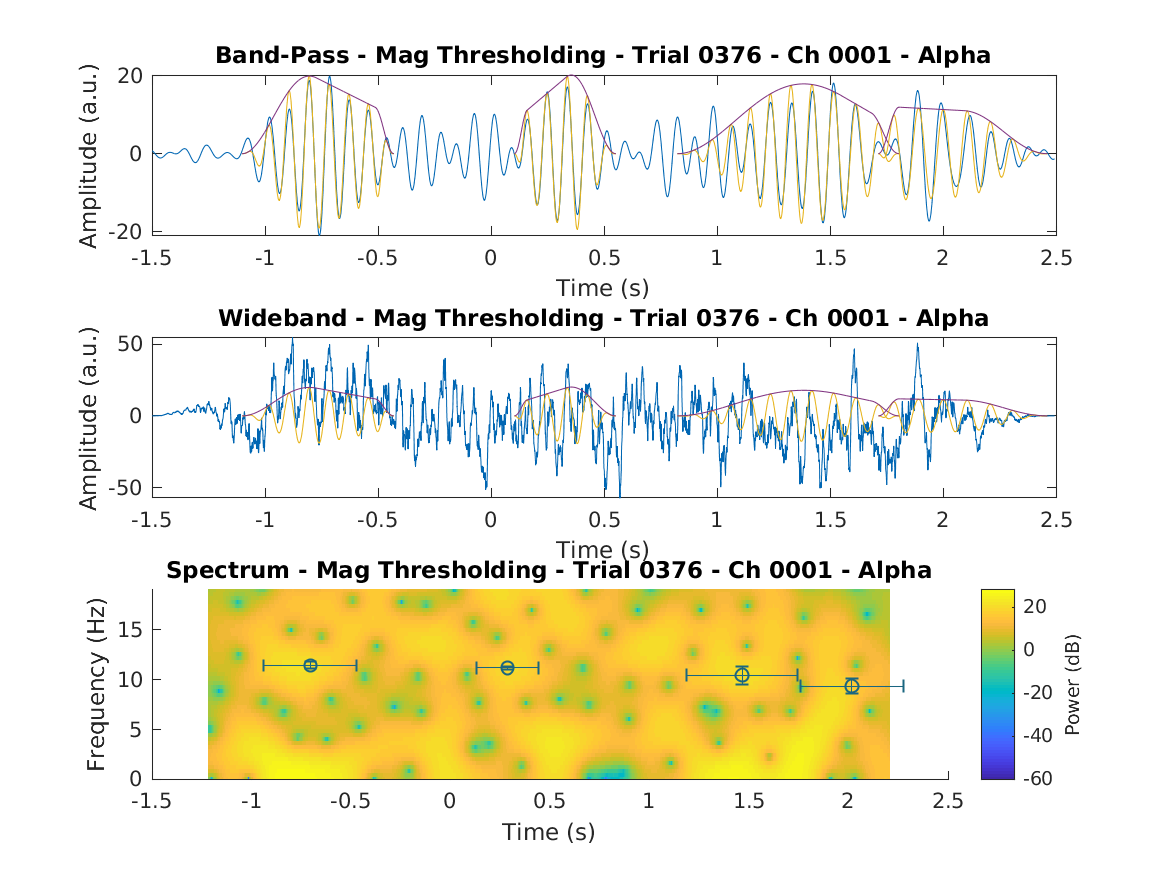
\includegraphics[height=3.5in]{plots3/commonwb-mag-tr0376-ch0001-al.png}
\end{center}}
{Field Trip data - typical detected events (alpha).}
{fig-tutor-ft1}

\figdef{\begin{center}
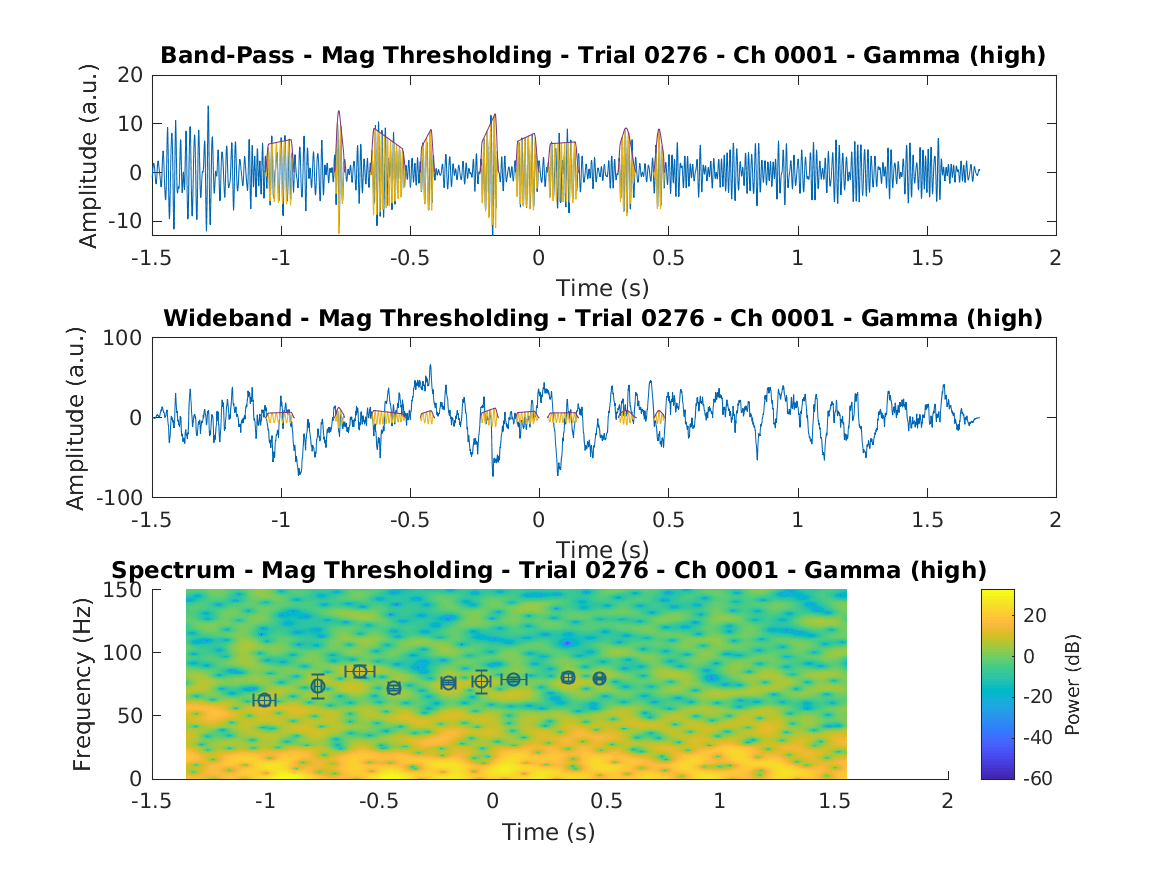
\includegraphics[height=3.5in]{plots3/commonwb-mag-tr0276-ch0001-gh.png}
\end{center}}
{Field Trip data - typical detected events (gamma).}
{fig-tutor-ft2}

%
%
\clearpage
\input{wlburst-guide-mincode-ft}
\clearpage

%
%
%
\section{Creating and Processing Synthetic Data}
\label{sect-tutor-synth}

A minimal script for creating synthetic neural data, detecting burst events,
and comparing detected events to ground truth is given in Section
\ref{sect-tutor-synthcode}. Steps that it performs are described below:

\begin{itemize}
%
\item Libraries are added to the path.
%
\item Frequency bands of interest are defined.

The structure format used for this follows the same conventions as the
``\texttt{bandinfo}'' structure array in \texttt{WLNOTES.txt}.
%
\item Segmentation and parameter extraction configuration structures are
created. These use the conventions described in \texttt{SEGCONFIG.txt}
and \texttt{PARAMCONFIG.txt}, respectively.
%
\item Detection threshold levels for a brute-force threshold sweep are
defined, as are per-band hand-tuned detection thresholds.
%
\item Per-band overrides for segmentation and parameter extraction are
defined, per \linebreak \texttt{wlFT\_doFindEventsInTrials\_MT.m}.
%
\item Synthetic neural data is generated via a call to
\texttt{wlSynth\_genFieldTrip}, using an array of parameter
specification structures to define many different types of event. Ground
truth for this synthetic data is also recorded.
%
\item Event detection is performed via calls to
\texttt{wlFT\_doFindEventsInTrials\_MT} (using magnitude-threshold detection),
with the detection threshold swept across a range of values. Post-processing
is applied (via \texttt{wlFT\_calcEventErrors} and
\texttt{wlAux\_pruneMatrix}) to remove putative events with waveforms that
don't match the band-pass-filtered input signal.
%
The output of this step is a cell array of event matrices, indexed by
threshold.
%
\item A ``selected'' event matrix is constructed using per-band detected
event lists corresponding to the per-band hand-tuned thresholds.
%
\item False positive, false negative, and true positive detection rates are
computed for each threshold in the threshold-sweep results, via
\texttt{wlFT\_compareMatrixEventsVsTruth}.
%
\item Plots are generated for the following data:
%
\begin{itemize}
\item Ground truth events in each trial are plotted against their trial
waveforms.
\item Detected events with hand-tuned thresholds are plotted against their
trial waveforms.
\item False positive and true positive rates (and counts) are plotted
as a function of threshold.
\item Curve fit parameters for detected events with hand-tuned thresholds
are scatter-plotted.
\end{itemize}
%
Several hundred trials are present, so the ``trial stride'' argument is used
to plot only the first trial out of every 25, for demonstration purposes.
%
\end{itemize}

Typical plots generated by this script are shown in Figures
\ref{fig-tutor-synth-gt} through \ref{fig-tutor-synth-scatter}.

\figdef{\begin{center}
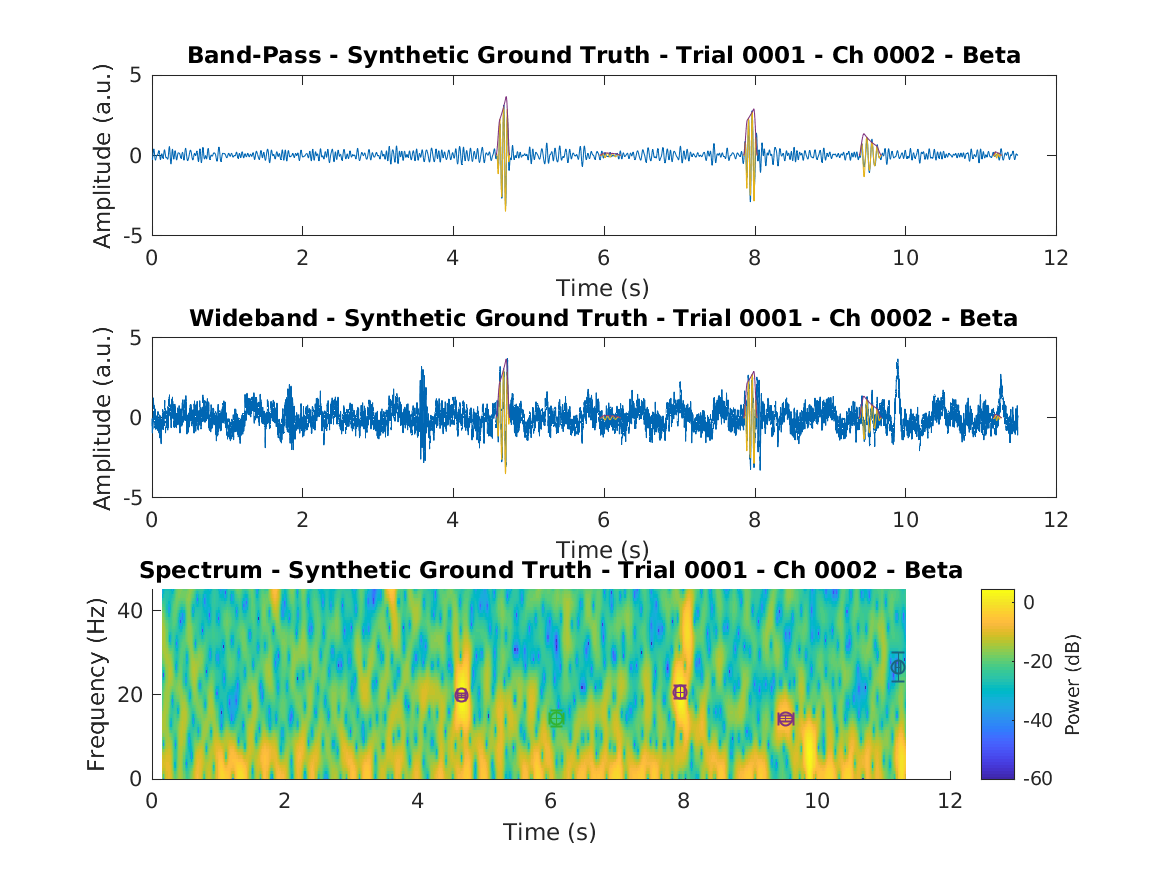
\includegraphics[height=3.5in]{plots3/commonwb-synthgt-tr0001-ch0002-be.png}
\end{center}}
{Synthetic data - typical ground truth events.}
{fig-tutor-synth-gt}

\figdef{\begin{center}
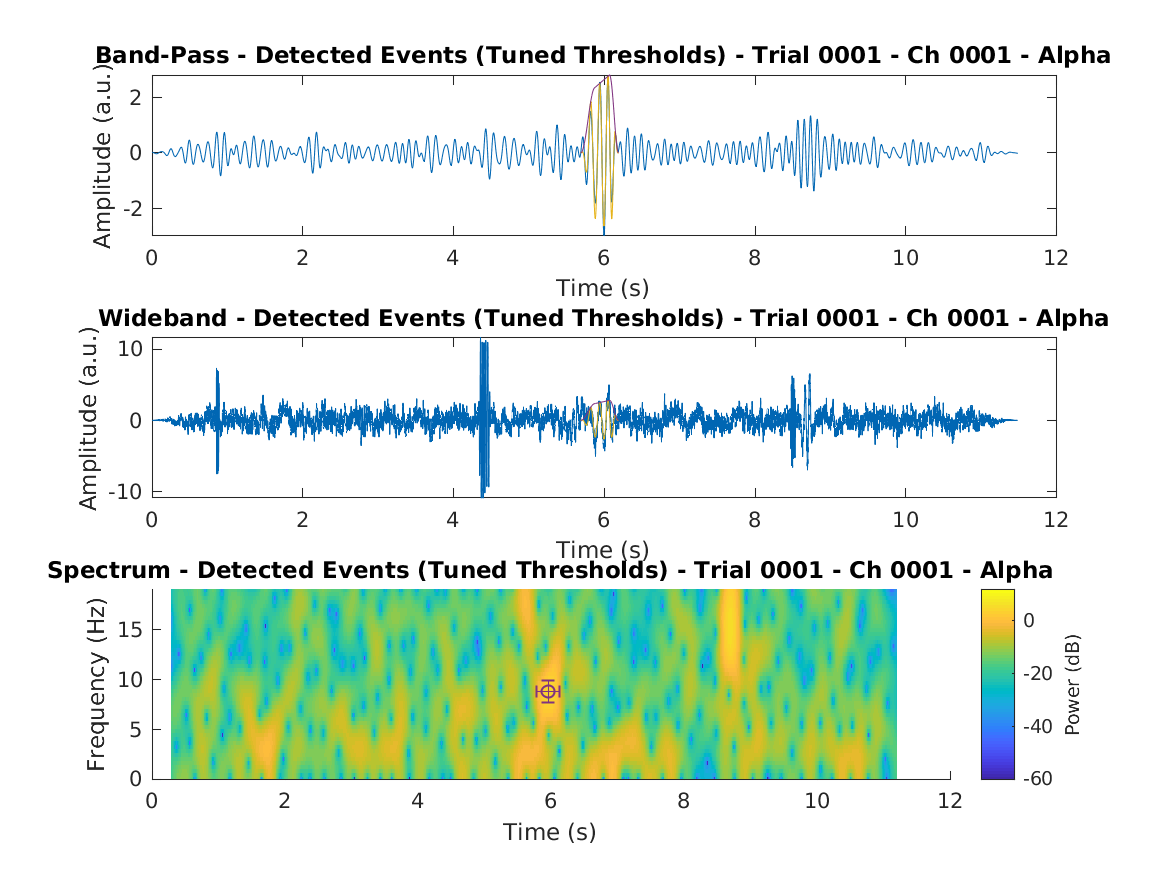
\includegraphics[height=3.5in]{plots3/commonwb-synthdet-tr0001-ch0001-al.png}
\end{center}}
{Synthetic data - typical detected events.}
{fig-tutor-synth-detect}

\figdef{\begin{center}
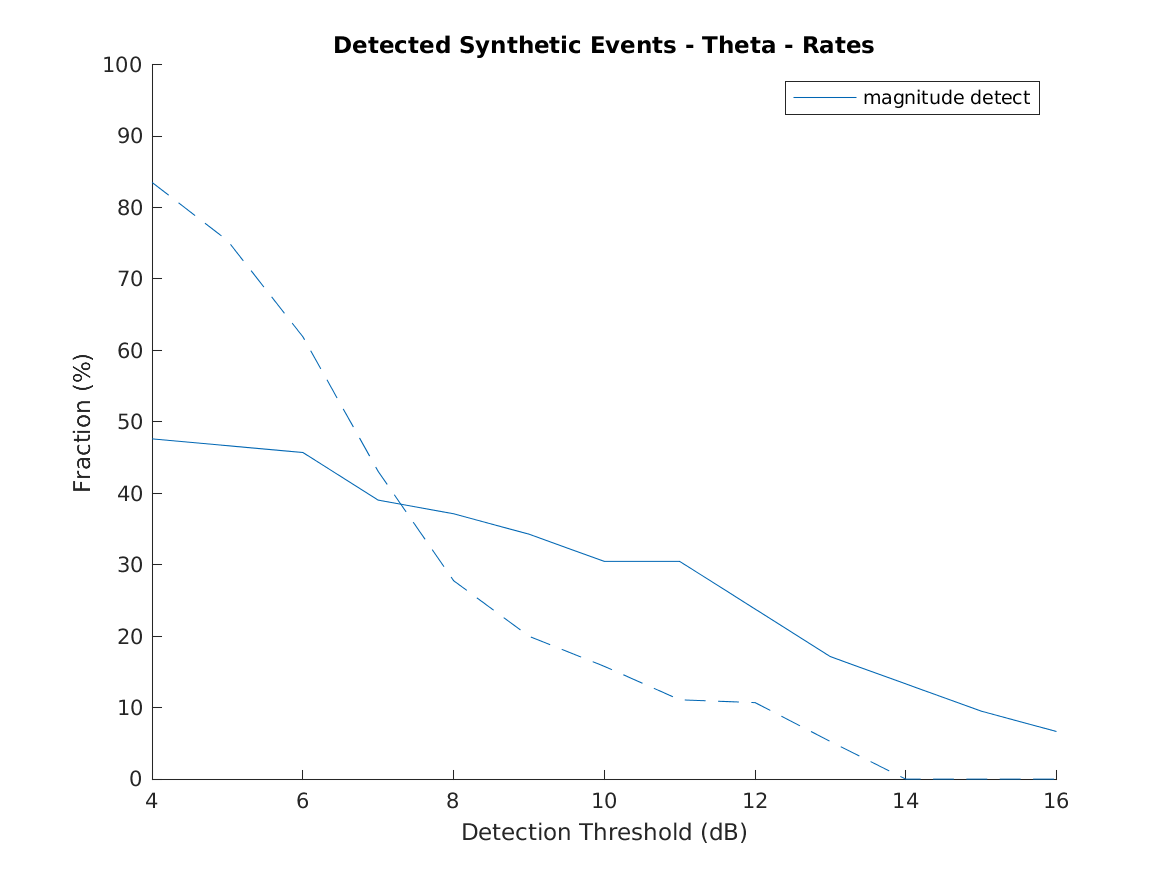
\includegraphics[height=3.5in]{plots3/detrate-thresh-th.png}
\end{center}}
{Synthetic data - typical detection rates vs threshold curve. The solid line
is the fraction of ground truth events detected; the dashed line is the
fraction of reported events that were false positives.}
{fig-tutor-synth-rates}

\figdef{\begin{center}
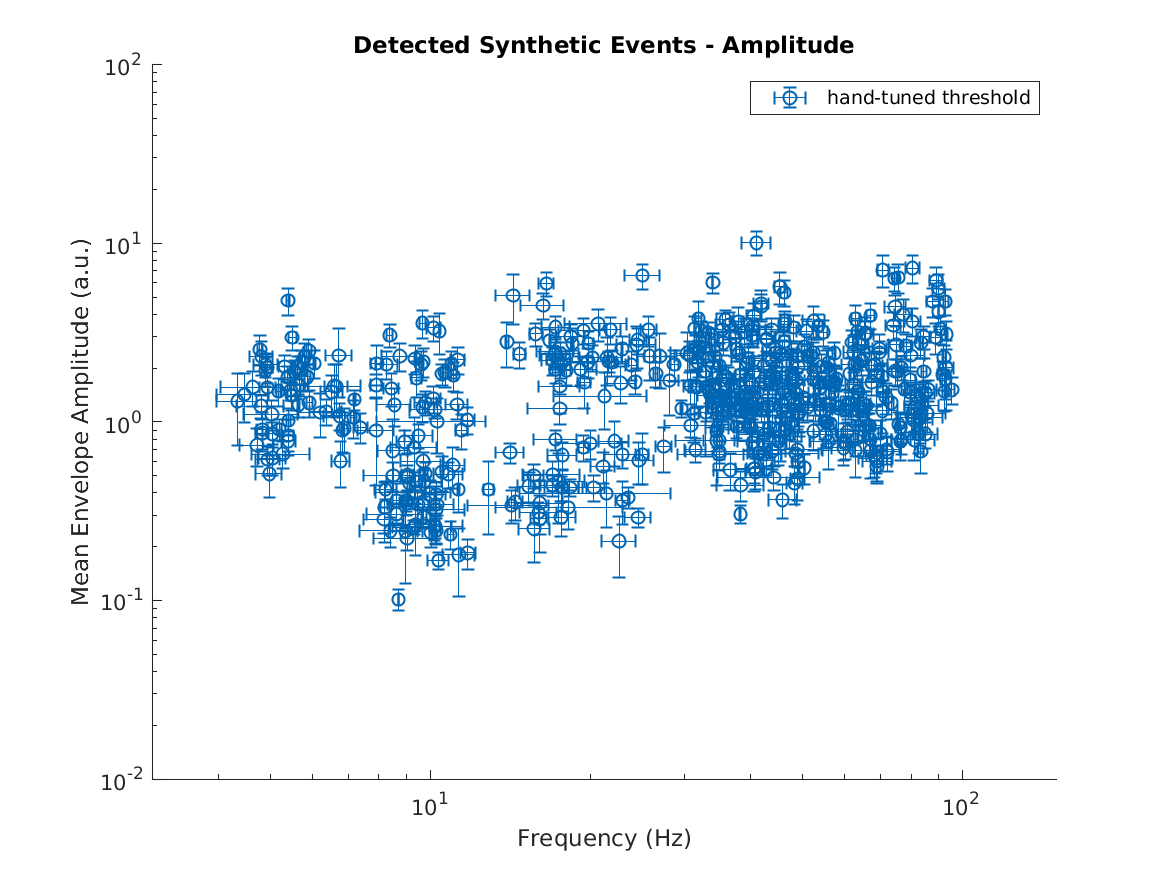
\includegraphics[height=3.5in]{plots3/evmult-amp-synthdet.png}
\end{center}}
{Synthetic data - scatter-plot of detected amplitude vs detected frequency.}
{fig-tutor-synth-scatter}

%
%
\clearpage
\input{wlburst-guide-mincode-synth}
\clearpage


%
% This is the end of the file.
